% Options for packages loaded elsewhere
% Options for packages loaded elsewhere
\PassOptionsToPackage{unicode}{hyperref}
\PassOptionsToPackage{hyphens}{url}
\PassOptionsToPackage{dvipsnames,svgnames,x11names}{xcolor}
%
\documentclass[
  10pt,
  letterpaper,
  DIV=11,
  numbers=noendperiod]{scrartcl}
\usepackage{xcolor}
\usepackage{amsmath,amssymb}
\setcounter{secnumdepth}{5}
\usepackage{iftex}
\ifPDFTeX
  \usepackage[T1]{fontenc}
  \usepackage[utf8]{inputenc}
  \usepackage{textcomp} % provide euro and other symbols
\else % if luatex or xetex
  \usepackage{unicode-math} % this also loads fontspec
  \defaultfontfeatures{Scale=MatchLowercase}
  \defaultfontfeatures[\rmfamily]{Ligatures=TeX,Scale=1}
\fi
\usepackage{lmodern}
\ifPDFTeX\else
  % xetex/luatex font selection
\fi
% Use upquote if available, for straight quotes in verbatim environments
\IfFileExists{upquote.sty}{\usepackage{upquote}}{}
\IfFileExists{microtype.sty}{% use microtype if available
  \usepackage[]{microtype}
  \UseMicrotypeSet[protrusion]{basicmath} % disable protrusion for tt fonts
}{}
% Make \paragraph and \subparagraph free-standing
\makeatletter
\ifx\paragraph\undefined\else
  \let\oldparagraph\paragraph
  \renewcommand{\paragraph}{
    \@ifstar
      \xxxParagraphStar
      \xxxParagraphNoStar
  }
  \newcommand{\xxxParagraphStar}[1]{\oldparagraph*{#1}\mbox{}}
  \newcommand{\xxxParagraphNoStar}[1]{\oldparagraph{#1}\mbox{}}
\fi
\ifx\subparagraph\undefined\else
  \let\oldsubparagraph\subparagraph
  \renewcommand{\subparagraph}{
    \@ifstar
      \xxxSubParagraphStar
      \xxxSubParagraphNoStar
  }
  \newcommand{\xxxSubParagraphStar}[1]{\oldsubparagraph*{#1}\mbox{}}
  \newcommand{\xxxSubParagraphNoStar}[1]{\oldsubparagraph{#1}\mbox{}}
\fi
\makeatother


\usepackage{longtable,booktabs,array}
\usepackage{calc} % for calculating minipage widths
% Correct order of tables after \paragraph or \subparagraph
\usepackage{etoolbox}
\makeatletter
\patchcmd\longtable{\par}{\if@noskipsec\mbox{}\fi\par}{}{}
\makeatother
% Allow footnotes in longtable head/foot
\IfFileExists{footnotehyper.sty}{\usepackage{footnotehyper}}{\usepackage{footnote}}
\makesavenoteenv{longtable}
\usepackage{graphicx}
\makeatletter
\newsavebox\pandoc@box
\newcommand*\pandocbounded[1]{% scales image to fit in text height/width
  \sbox\pandoc@box{#1}%
  \Gscale@div\@tempa{\textheight}{\dimexpr\ht\pandoc@box+\dp\pandoc@box\relax}%
  \Gscale@div\@tempb{\linewidth}{\wd\pandoc@box}%
  \ifdim\@tempb\p@<\@tempa\p@\let\@tempa\@tempb\fi% select the smaller of both
  \ifdim\@tempa\p@<\p@\scalebox{\@tempa}{\usebox\pandoc@box}%
  \else\usebox{\pandoc@box}%
  \fi%
}
% Set default figure placement to htbp
\def\fps@figure{htbp}
\makeatother





\setlength{\emergencystretch}{3em} % prevent overfull lines

\providecommand{\tightlist}{%
  \setlength{\itemsep}{0pt}\setlength{\parskip}{0pt}}



 


\usepackage{xcolor, soul}
\definecolor{Light}{gray}{.90}
\sethlcolor{Light}
\let\OldTexttt\texttt
\renewcommand{\texttt}[1]{\OldTexttt{\hl{#1}}}
\usepackage{caption}
\captionsetup{font=small, labelfont=bf}
\setlength{\parindent}{0pt}
\setlength{\parskip}{1.25ex}
\KOMAoption{captions}{tableheading}
\makeatletter
\@ifpackageloaded{caption}{}{\usepackage{caption}}
\AtBeginDocument{%
\ifdefined\contentsname
  \renewcommand*\contentsname{Table of contents}
\else
  \newcommand\contentsname{Table of contents}
\fi
\ifdefined\listfigurename
  \renewcommand*\listfigurename{List of Figures}
\else
  \newcommand\listfigurename{List of Figures}
\fi
\ifdefined\listtablename
  \renewcommand*\listtablename{List of Tables}
\else
  \newcommand\listtablename{List of Tables}
\fi
\ifdefined\figurename
  \renewcommand*\figurename{Figure}
\else
  \newcommand\figurename{Figure}
\fi
\ifdefined\tablename
  \renewcommand*\tablename{Table}
\else
  \newcommand\tablename{Table}
\fi
}
\@ifpackageloaded{float}{}{\usepackage{float}}
\floatstyle{ruled}
\@ifundefined{c@chapter}{\newfloat{codelisting}{h}{lop}}{\newfloat{codelisting}{h}{lop}[chapter]}
\floatname{codelisting}{Listing}
\newcommand*\listoflistings{\listof{codelisting}{List of Listings}}
\makeatother
\makeatletter
\makeatother
\makeatletter
\@ifpackageloaded{caption}{}{\usepackage{caption}}
\@ifpackageloaded{subcaption}{}{\usepackage{subcaption}}
\makeatother
\usepackage{bookmark}
\IfFileExists{xurl.sty}{\usepackage{xurl}}{} % add URL line breaks if available
\urlstyle{same}
\hypersetup{
  pdftitle={Detection of sparsity in neural responses},
  pdfauthor={Al Xin},
  colorlinks=true,
  linkcolor={blue},
  filecolor={Maroon},
  citecolor={Blue},
  urlcolor={Blue},
  pdfcreator={LaTeX via pandoc}}


\title{Detection of sparsity in neural responses}
\author{\small Al Xin}
\date{Aug 17, 2026}
\begin{document}
\maketitle


\section{Motivation}\label{motivation}

Very few investigators record visual texture responses from IT due to
the lack of a strong, coherent response. \emph{A priori}, we should
expect a sparse response in IT. There are a few ways that sparseness may
appear in IT:

\begin{enumerate}
\def\labelenumi{\arabic{enumi}.}
\tightlist
\item
  There are a few IT neurons whose responses to the texture families
  tend to be strong and reliable.
\item
  For each texture family, there are a few neurons whose response is
  reliable, but the responsive neurons for each family may differ.
\item
  For some texture families, there are a few neurons whose response is
  reliable.
\item
  Same as (3), but for each specific image (sample ID).
\item
  Same as (3), but for each specific image.
\end{enumerate}

Because reliable sites are identified by correlation to the same
stimuli, it is possible to consistently miss patterns of sparsity
outside of (1). In this new analysis, I want to visualize the
reliability of neurons in a way that is not dependent on the previous
criteria for reliable site. Furthermore, I want to compare this approach
across all regions recorded. Since scenario (5) is most general, we want
to focus on approaches to characterize the neural response that would
work in this situation.

\section{Plan}\label{plan}

The most basic analysis is to perform a two sample t-test for each
neuron's response for a specific image compared to the response to blank
images. Since there are 6 repetitions, this should work well enough.
Furthermore, it would be useful to visualize each component of the
t-test. For example, if in IT, we may see that the difference in means
for samples in a family tend to be consistently positive but the
differences are not significant due to higher variance. This may
indicate that there is some response at the family level and that we
could detect a significant difference if the trials were pooled at the
family level rather than the specific image level. Regardless, it would
be worthwhile to do this analysis both at the specific image level and
the texture family level.

\section{Data}\label{data}

See \texttt{20260625.qmd} for reference for how data were processed.
Note that the window of averaged responses depends on the criteria for
reliability. For now, I will proceed with the already calculated
average, but note this potential source of bias, especially for IT which
does not have many reliable sites.

Unlike the previous notebooks, analysis will be \emph{not} be limited to
reliable sites. For now, we will still only consider images with
naturalistic structure compared to blank images.

\section{Methods}\label{methods}

\subsection{Two-sample t-test}\label{two-sample-t-test}

To compare the mean firing between blank and non-blank images, Welch's
\emph{t}-test will be used. The statistic \emph{t} is found as \[
t = \frac
{ \overline{X}_1 - \overline{X}_2 }
{ \sqrt{s^2_{\overline{X}_1} + s^2_{\overline{X}_2}} }, 
\quad 
s_{\overline{X}_i} = \frac{s_i}{\sqrt{n_i}}
\] where \(\overline{X}_i\) is the sample mean, and
\(s_{\overline{X}_i}\) is the standard error, \(s_i\) is the sample
standard deviation, and \(n_i\) is the sample size. The
\emph{t}-distribution's degrees of freedom can be approximated as \[
\nu \approx \frac
{ \left( s^2_{\overline{X}_1} + s^2_{\overline{X}_2} \right)^2 }
{ \frac{s^4_{\overline{X}_1}}{n_1 - 1} + \frac{s^4_{\overline{X}_2}}{n_2 - 1} }.
\] For simplicity, this will be implemented by \texttt{t.test()}.

\section{Results}\label{results}

\subsection{Blank image baseline
response}\label{blank-image-baseline-response}

The average response and the standard deviation of response to blank
images will be pooled over all the repetitions of blank images, of which
there are 600 for each session. The blank images are labeled by ID (1 to
100) and repetitions (1 to 6), though I believe this is arbitrary.
Density plots of the mean blank responses and the standard error of
blank responses for each site and region are displayed in
Figure~\ref{fig-blanks}. V1 responses tend to exhibit lower standard
deviations and lower mean firing rate, but the differences between V2,
V4, and IT are less noticeable. V2 seems to have more variable mean
firing in response to blank images.

\begin{figure}

\centering{

\pandocbounded{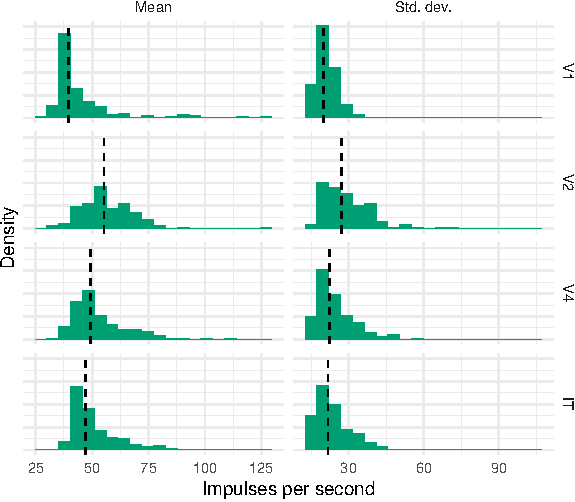
\includegraphics[keepaspectratio]{20260813_files/figure-pdf/fig-blanks-1.pdf}}

}

\caption{\label{fig-blanks}Histogram of the mean response to blank
images and SE of response to blank images for each region. The number of
observations differs for each region, so the y-axis has been replaced
with density rather than count. Dashed lines indicate the median. V1
shows lower mean firing rates and standard deviations.}

\end{figure}%

\subsection{Qualitative per-site response to
images}\label{qualitative-per-site-response-to-images}

\subsubsection{Distribution when pooled over non-blank
images}\label{distribution-when-pooled-over-non-blank-images}

The per-site mean and standard deviations for firings for all non-blank
images (pooled) can be seen in the left of Figure~\ref{fig-imgs}. The
means are reported as the difference with the blank images. The spread
of the mean difference for IT is very narrow with a lower median than
the other regions. The high mean difference for V2 is consistent with
previous work. V1 and V4 are comparable, which is somewhat surprising
considering previous work by Lee et al.~showing that coding for
naturalistic texture families is stronger in V4. These results could
still be consistent if the noisy textures produce much smaller average
responses in V4, though we are not necessarily examining this currently.

\subsubsection{Distribution when pooled over specific image
repetitions}\label{distribution-when-pooled-over-specific-image-repetitions}

Figure~\ref{fig-imgs} (right) contains the difference in means and the
standard deviations for the specific images, so pooling is only done
over repetitions. With more data points, the distributions tend to look
less irregular overall, though the trends in the medians are similar to
when pooling is performed over the sites in \textbf{?@fig-sites}. The
distribution of the difference in means for IT appears shifted to the
left and more centered around zero.

\begin{figure}

\centering{

\pandocbounded{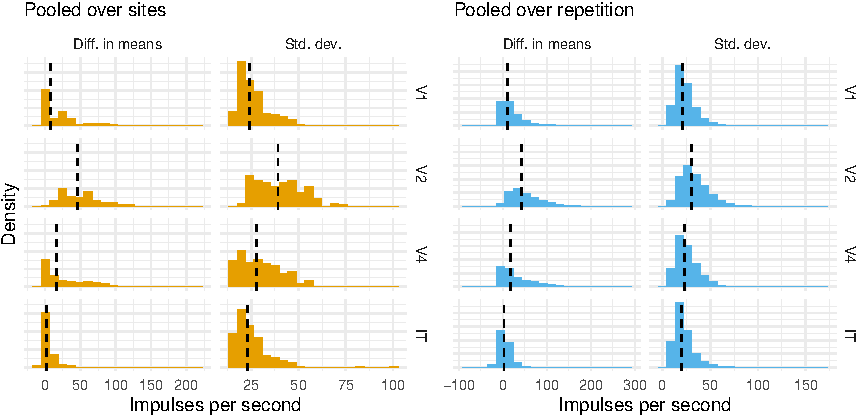
\includegraphics[keepaspectratio]{20260813_files/figure-pdf/fig-imgs-1.pdf}}

}

\caption{\label{fig-imgs}(Left) Densities of the mean response
(difference with blank images) and standard deviations of responses to
pooled non-blank images for each region. Dashed lines indicate the
median. IT shows lower and less variable differences in mean firing rate
and lower standard deviations. (Right) Results with pooling only over
repetition. The overall trends are similar to the left plot, though the
IT differences in means seem more centered around zero.}

\end{figure}%

\subsubsection{Firing in specific combinations of site and
image}\label{firing-in-specific-combinations-of-site-and-image}

In Figure~\ref{fig-heatmaps}, the heat map of mean differences and
standard deviations helps visualize the per-site and per-image
distribution of firing patterns. Even with this basic visualization, the
divisions between each array tend to be clear, with the exception of V2.
For instance, in V4, the second array (i.e., the 96 columns in the
center of the heat maps) shows markedly lower differences in means and
standard errors.

As a heuristic, vertical striping in the heat maps indicates per-site
differences and horizontal striping in the heat maps indicates per-image
differences. V2 and V4 show more between-site and between-image
variation, consistent with previous results on decoding texture families
in these regions.

\begin{figure}

\centering{

\pandocbounded{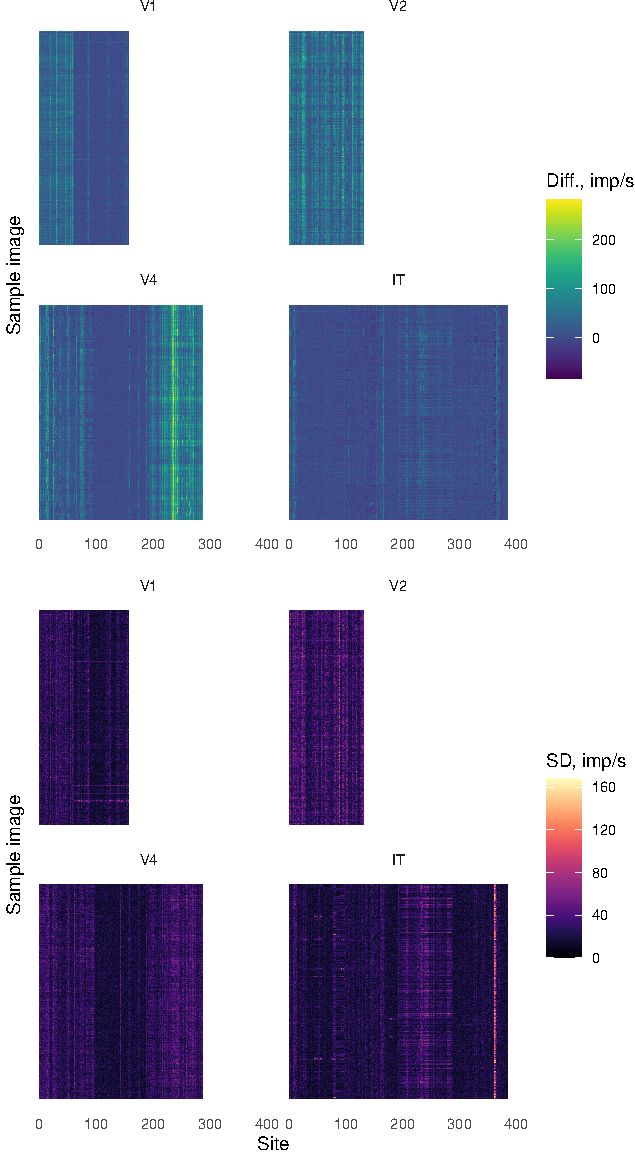
\includegraphics[keepaspectratio]{20260813_files/figure-pdf/fig-heatmaps-1.pdf}}

}

\caption{\label{fig-heatmaps}(Top) Heat map of the differences in means
between sample images and the blank images for each site. (Bottom)
Standard deviations in firing over repetitions of each sample image for
each site. V2 and V4 show more between-site and between-image variation
in firing patterns.}

\end{figure}%

\subsection{Two sample t-test results}\label{two-sample-t-test-results}

The heat map of \emph{t-}-statistics (top) and \emph{p}-values from the
\emph{t}-tests in Figure~\ref{fig-t_tests} displays similar information

\begin{figure}

\centering{

\pandocbounded{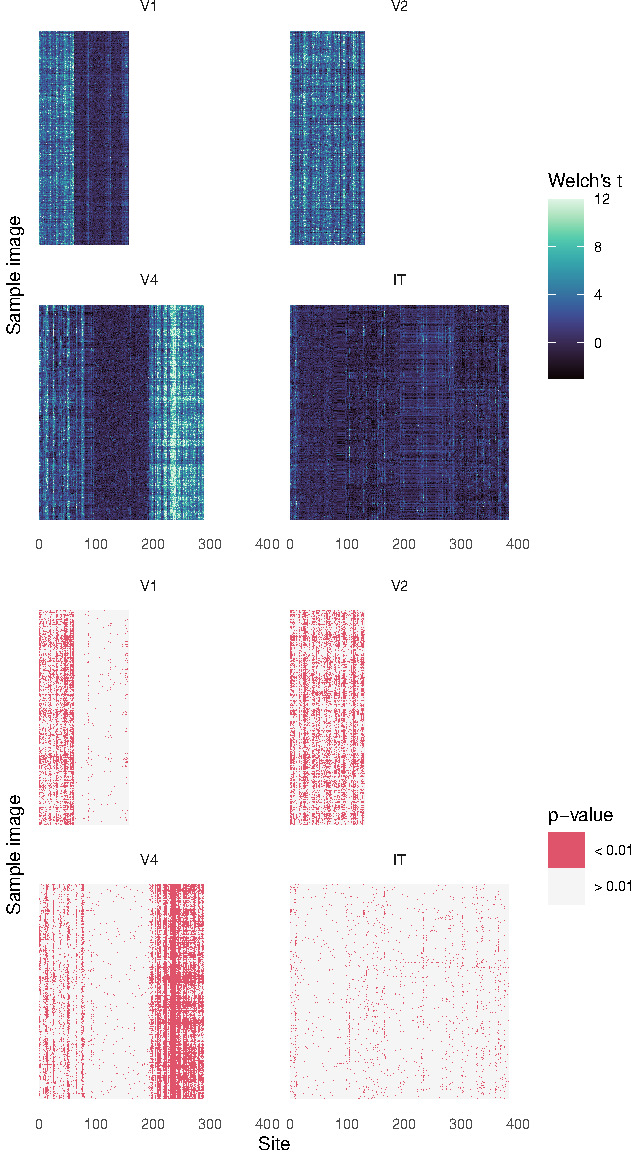
\includegraphics[keepaspectratio]{20260813_files/figure-pdf/fig-t_tests-1.pdf}}

}

\caption{\label{fig-t_tests}(Top) Heat map of the t-statistics
calculated for each combination of site and image. The degrees of
freedom are identical fir eacg test. The scale has been truncated to
(-3, 12). (Bottom) Corresponding p-values, simplified to indicate
whether values are below or above a cutoff of 0.01. The graphs are
similar to the difference in means plots, though the p-value plot more
clearly shows the vertical, per-site firing consistency in V4 and the
sparseness in IT.}

\end{figure}%




\end{document}
